% Kap. 2 -- Neuaufbau 2026-11-05, Stil "luftig" 2026-11-06 (Backup: ../elektronik-1_backup_2026-11-05)
\section{Operationsverstärker}\label{sec:opamp}

\subsection{Idealer OpAmp und Arbeitsbereich}\label{sec:opamp-ideal}

\begin{minipage}[c]{0.42\columnwidth}
	\centering
	\resizebox{\columnwidth}{!}{% LTeX: enabled=false
\resizebox{0.6\columnwidth}{!}{
    \begin{circuitikz}
        \tikzstyle{every node}=[font=\Huge]
        \draw [line width=1pt, short] (0,0) -- (7.75,4.5);
        \draw [line width=1pt, short] (0,0) -- (0,9);
        \draw (4.25,4.5) to[american voltage source] (2.75,3);
        \draw [line width=1pt, short] (7.75,4.5) -- (0,9);
        \node at (1,2.5) {\textbf{+}};
        \node at (1,6.5) {\textbf{-}};
        \draw (0.5,2.5) to[european resistor] (0.5,6.5);
        \draw (0.5,2.5) to[short, -o] (-1.75,2.5) ;
        \draw (0.5,6.5) to[short, -o] (-1.75,6.5) ;
        \draw [<->, >=Stealth] (-0.5,2.5) -- (-0.5,6.5)node[pos=0.5, fill=white]{$V_{in}$};
        \node at (1.75,4.5) {$Z_i = \infty$};
        \draw (2.75,3) to (2.75,2.75) node[ground]{};
        \node at (4.5,3.25) {$a = \infty$};
        \draw (4.25,4.5) to[european resistor] (6,4.5);
        \draw (6,4.5) to[short, -o] (9,4.5) ;
        \draw [->, >=Stealth] (-2,2) -- (-0.25,2)node[pos=0.5, fill=white]{$I_{in}=0$};
        \node at (8.5,5) {$V_{out}$};
        \draw [->, >=Stealth] (-1.75,7) -- (-0.25,7)node[pos=0.5, fill=white]{$I_{in}=0$};
        \node at (5,5) {$Z_{out} = 0$};
    \end{circuitikz}
}%
%Tikzmaker code:
%[[],[{"x":0,"y":850},{"x":387.5,"y":625},"Line",1,"\\draw [line width=1pt, short] (0,0) -- (7.75,4.5);","",[0,0,0],[255,255,255],0,false,[0,0,0,0],1,{"fontSize":32,"textPlacement":0.5,"isBold":false,"isItalic":false,"hasUnderline":false,"alignmentText":"center"}],[{"x":0,"y":850},{"x":0,"y":400},"Line",3,"\\draw [line width=1pt, short] (0,0) -- (0,9);","",[0,0,0],[255,255,255],0,false,[0,0,0,0],1,{"fontSize":32,"textPlacement":0.5,"isBold":false,"isItalic":false,"hasUnderline":false,"alignmentText":"center"}],[{"x":212.5,"y":625},{"x":137.5,"y":700},"Voltage Source (American)",5,"\\draw (4.25,4.5) to[american voltage source] (2.75,3);","",[0,0,0],[255,255,255],0,false,32,0.4,{"isBold":false,"isItalic":false,"hasUnderline":false,"rotation":0,"frequency":1,"amplitude":1,"phase":0,"multiwire":0,"alignmentText":"center","endNodeType":"circ"}],[{"x":387.5,"y":625},{"x":0,"y":400},"Line",7,"\\draw [line width=1pt, short] (7.75,4.5) -- (0,9);","",[0,0,0],[255,255,255],0,false,[0,0,0,0],1,{"fontSize":32,"textPlacement":0.5,"isBold":false,"isItalic":false,"hasUnderline":false,"alignmentText":"center"}],[{"x":50,"y":725},{"x":50,"y":725},"Text",8,"\\node [font=\\LARGE] at (1,2.5) {\\textbf{+}};","+",[0,0,0],[255,255,255],0,false,32,0.4,{"isBold":true,"isItalic":false,"hasUnderline":false,"rotation":0,"frequency":1,"amplitude":1,"phase":0,"multiwire":0,"alignmentText":"center","endNodeType":"circ","isMathMode":false}],[{"x":50,"y":525},{"x":50,"y":525},"Text",9,"\\node [font=\\LARGE] at (1,6.5) {\\textbf{-}};","-",[0,0,0],[255,255,255],0,false,32,0.4,{"isBold":true,"isItalic":false,"hasUnderline":false,"rotation":0,"frequency":1,"amplitude":1,"phase":0,"multiwire":0,"alignmentText":"center","endNodeType":"circ","isMathMode":false}],[{"x":25,"y":725},{"x":25,"y":525},"Resistor (IEC)",10,"\\draw (0.5,2.5) to[european resistor] (0.5,6.5);","",[0,0,0],[255,255,255],0,false,32,0.4,{"isBold":false,"isItalic":false,"hasUnderline":false,"rotation":0,"frequency":1,"amplitude":1,"phase":0,"multiwire":0,"alignmentText":"center","endNodeType":"circ","isMathMode":true}],[{"x":25,"y":725},{"x":-87.5,"y":725},"End node",12,"\\draw [](0.5,2.5) to[short, -o] (-1.75,2.5) ;","",[0,0,0],[255,255,255],0,false,32,0.4,{"isBold":false,"isItalic":false,"hasUnderline":false,"rotation":0,"frequency":1,"amplitude":1,"phase":0,"multiwire":0,"alignmentText":"center","endNodeType":"circ"}],[{"x":25,"y":525},{"x":-87.5,"y":525},"End node",13,"\\draw [](0.5,6.5) to[short, -o] (-1.75,6.5) ;","",[0,0,0],[255,255,255],0,false,32,0.4,{"isBold":false,"isItalic":false,"hasUnderline":false,"rotation":0,"frequency":1,"amplitude":1,"phase":0,"multiwire":0,"alignmentText":"center","endNodeType":"circ"}],[{"x":-25,"y":725},{"x":-25,"y":525},"Double-headed arrow",14,"\\draw [<->, >=Stealth] (-0.5,2.5) -- (-0.5,6.5)node[pos=0.5,undefined, fill=white]{$V_{in}$};","V_{in}",[0,0,0],[255,255,255],0,false,[0,0,0,0],0.4,{"fontSize":32,"textPlacement":0.5,"isBold":false,"isItalic":false,"hasUnderline":false,"isMathMode":true}],[{"x":87.5,"y":625},{"x":87.5,"y":625},"Text",15,"\\node [font=\\Large] at (1.75,4.5) {$Z_i = \\infty$};","Z_i = \\infty",[0,0,0],[255,255,255],0,true,27,0.4,{"isBold":false,"isItalic":false,"hasUnderline":false,"isMathMode":true,"rotation":0}],[{"x":137.5,"y":700},{"x":137.5,"y":712.5},"Ground",16,"\\draw (2.75,3) to (2.75,2.75) node[ground]{};","",[0,0,0],[255,255,255],0,false,22,0.4,{"isBold":false,"isItalic":false,"hasUnderline":false,"isMathMode":true,"rotation":0,"frequency":1,"amplitude":1,"phase":0,"multiwire":0,"endNodeType":"circ"}],[{"x":212.5,"y":687.5},{"x":212.5,"y":687.5},"Text",19,"\\node [font=\\Large] at (4.25,3.25) {$a = \\infty$};","a = \\infty",[0,0,0],[255,255,255],0,false,27,0.4,{"isBold":false,"isItalic":false,"hasUnderline":false,"isMathMode":true,"rotation":0}],[{"x":212.5,"y":625},{"x":300,"y":625},"Resistor (IEC)",20,"\\draw (4.25,4.5) to[european resistor] (6,4.5);","",[0,0,0],[255,255,255],0,false,22,0.4,{"isBold":false,"isItalic":false,"hasUnderline":false,"isMathMode":true,"rotation":0,"frequency":1,"amplitude":1,"phase":0,"multiwire":0,"endNodeType":"circ"}],[{"x":300,"y":625},{"x":450,"y":625},"End node",23,"\\draw [](6,4.5) to[short, -o] (9,4.5) ;","",[0,0,0],[255,255,255],0,false,22,0.4,{"isBold":false,"isItalic":false,"hasUnderline":false,"isMathMode":true,"rotation":0,"frequency":1,"amplitude":1,"phase":0,"multiwire":0,"endNodeType":"circ"}],[{"x":-100,"y":750},{"x":-12.5,"y":750},"Arrow",24,"\\draw [->, >=Stealth] (-2,2) -- (-0.25,2)node[pos=0.5,undefined, fill=white]{$I_{in}=0$};","I_{in}=0",[0,0,0],[255,255,255],0,false,[0,0,0,0],0.4,{"fontSize":22,"textPlacement":0.5,"isBold":false,"isItalic":false,"hasUnderline":false,"isMathMode":true}],[{"x":425,"y":600},{"x":425,"y":600},"Text",26,"\\node [font=\\Large] at (8.5,5) {$V_{out}$};","V_{out}",[0,0,0],[255,255,255],0,false,27,0.4,{"isBold":false,"isItalic":false,"hasUnderline":false,"isMathMode":true,"rotation":0}],[{"x":-87.5,"y":500},{"x":-12.5,"y":500},"Arrow",27,"\\draw [->, >=Stealth] (-1.75,7) -- (-0.25,7)node[pos=0.5,undefined, fill=white]{$I_{in}=0$};","I_{in}=0",[0,0,0],[255,255,255],0,false,[0,0,0,0],0.4,{"fontSize":27,"textPlacement":0.5,"isBold":false,"isItalic":false,"hasUnderline":false,"isMathMode":true}],[{"x":250,"y":600},{"x":250,"y":600},"Text",28,"\\node [font=\\Large] at (5,5) {$Z_{out} = 0$};","Z_{out} = 0",[0,0,0],[255,255,255],0,false,27,0.4,{"isBold":false,"isItalic":false,"hasUnderline":false,"isMathMode":true,"rotation":0}]]}
\end{minipage}
\hfill
\begin{minipage}[c]{0.56\columnwidth}
	$$ \boxed{ V_{\rm out} = A_{\rm ol}\,(V_{\rm opp} + V_{\rm os} - V_{\rm opn}) } $$
	\textbf{Ideal}: \; $A_{\rm ol}\to\infty$, \; $I_{\rm opp}=I_{\rm opn}=0$, \; $Z_{\rm out}=0$, \; $V_{\rm os}=0$
\end{minipage}

\vspace{4pt}
{\renewcommand{\arraystretch}{1.45}
\begin{tabularx}{\columnwidth}{@{}l X@{}}
	\toprule
	\textbf{Situation}        & \textbf{Was gilt} \\ \midrule
	Gegenkopplung auf opn     & $V_{\rm opn} = V_{\rm opp}$ (virtueller Kurzschluss), \; $I_{R_{\rm in}} = I_{R_f}$ \\
	Ohne Gegenkopplung        & Ausgang am Anschlag: $V_{\rm opp} > V_{\rm opn} \Rightarrow V_{\rm out,max}$, sonst $V_{\rm out,min}$ \\
	$Z_{\rm out} = 0$         & Last $R_L$ ändert $V_{\rm out}$ nicht \\
	Ausgangsbereich           & $V_{\rm out,min} \le V_{\rm out} \le V_{\rm out,max}$ \; (Rail-to-Rail: $V_{\rm SS}\dots V_{\rm DD}$) \\
	Eingangsbereich           & P-Stufe: $V_{\rm SS}\dots V_{\rm DD}{-}1\,$V; \; N-Stufe: $1\,{\rm V}\dots V_{\rm DD}$ \\ \bottomrule
\end{tabularx}}

\warn{\textit{Se il risultato esce dai rail, l'uscita resta al rail: il calcolo lineare non vale più.}}

\subsection{Rezept: $V_{\rm out} = \sum a_i V_i + b$}\label{sec:opamp-rezept}

\begin{rezept}{Rezept: OpAmp-Schaltung mit mehreren Quellen}
	\begin{steps}
		\item $V_{\rm opp}$ bestimmen: Spannungsteiler / Superposition aller Quellen am $+$-Eingang
		\item Jede Quelle $V_i$, die über $R_i$ an opn hängt (alle anderen Quellen $=0$):
		      \; $a_i = -\dfrac{R_f}{R_i}$
		\item \textbf{Noise Gain}: $R_\parallel$ = \textbf{alle} Widerstände von opn zu Quellen, AGND, GND parallel
	\end{steps}
	$$ G_N = \frac{1}{\beta} = 1 + \frac{R_f}{R_\parallel} \qquad\quad
	   \beta = \frac{V_{\rm opn}}{V_{\rm out}}\bigg|_{\text{Quellen}=0} = \frac{R_\parallel}{R_\parallel + R_f} $$
	$$ \boxed{ V_{\rm out} = G_N \,(V_{\rm opp} + V_{\rm os}) - \sum_i \frac{R_f}{R_i}\,V_i } $$
	\textbf{Kontrolle}: alle Quellen $= V_{\rm AGND}$ \textrightarrow\ $V_{\rm out} = V_{\rm AGND}$ (bei symmetrischen Teilern)
\end{rezept}

\subsection{Grundschaltungen (ideal, mit $V_{\rm os}$)}\label{sec:opamp-grund}

{\renewcommand{\arraystretch}{1.5}
\begin{tabularx}{\columnwidth}{@{}p{0.25\columnwidth} X@{}}
	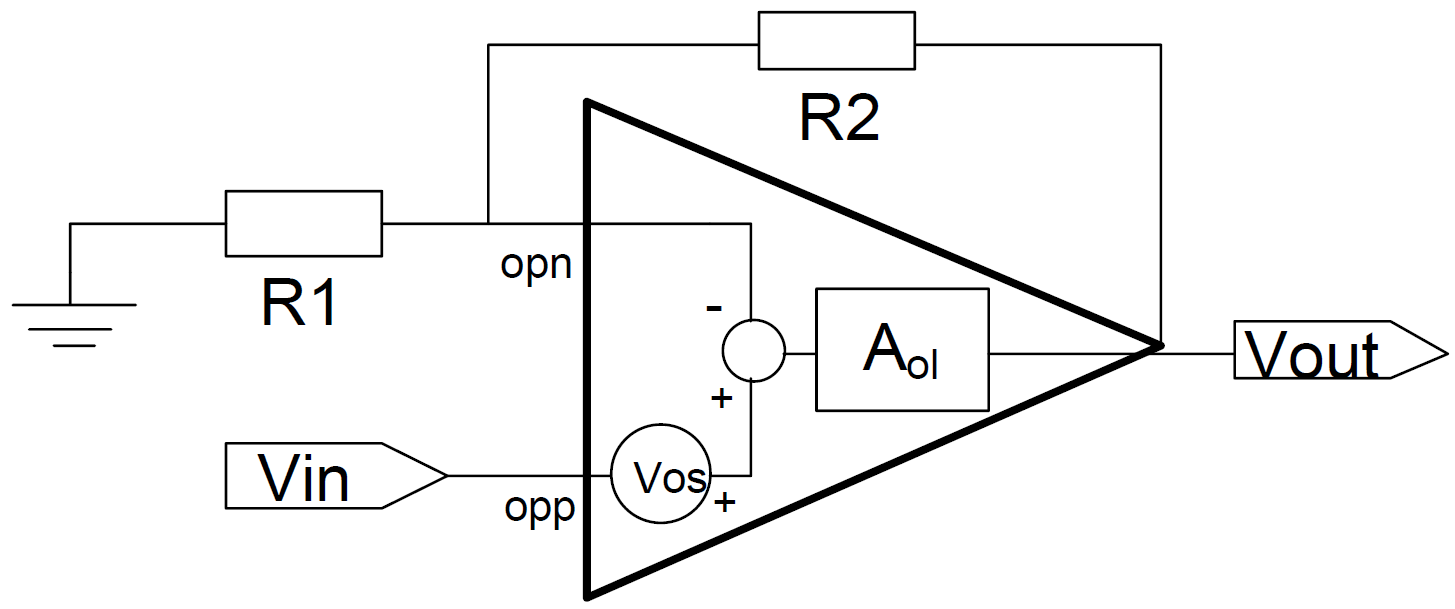
\includegraphics[width=\linewidth,align=c]{images/nicht-invertierender_verstaerker_offset.png} &
	\textbf{Nicht-invertierend} \quad $Z_{\rm in}=\infty$, \; $G_N = 1+\frac{R_2}{R_1}$ \newline
	$V_{\rm out} = \Big(1+\dfrac{R_2}{R_1}\Big)(V_{\rm in}+V_{\rm os}) - \dfrac{R_2}{R_1}V_{\rm AGND}$ \\
	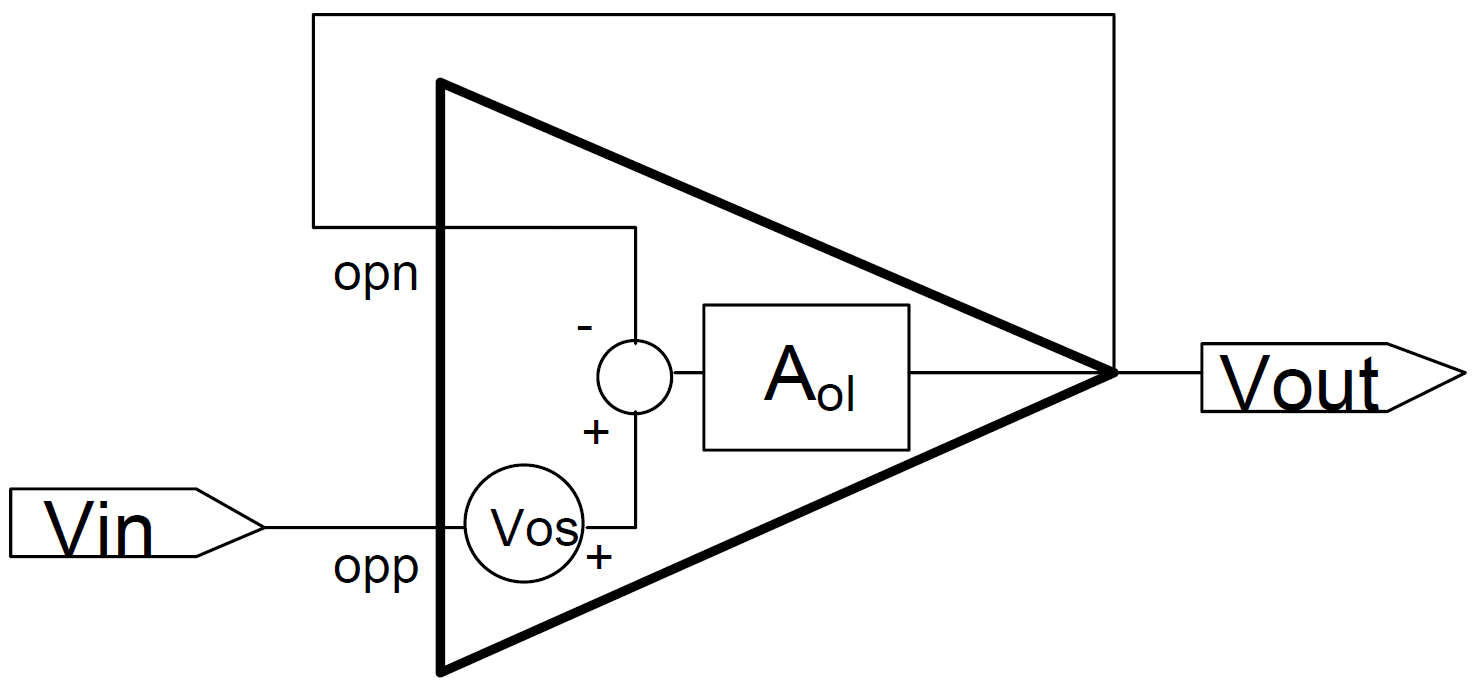
\includegraphics[width=0.8\linewidth,align=c]{images/buffer_offset.png} &
	\textbf{Buffer} (Impedanzwandler) \quad $Z_{\rm in}=\infty$, \; $Z_{\rm out}=0$, \; $G_N=1$ \newline
	$V_{\rm out} = V_{\rm in} + V_{\rm os}$ \\
	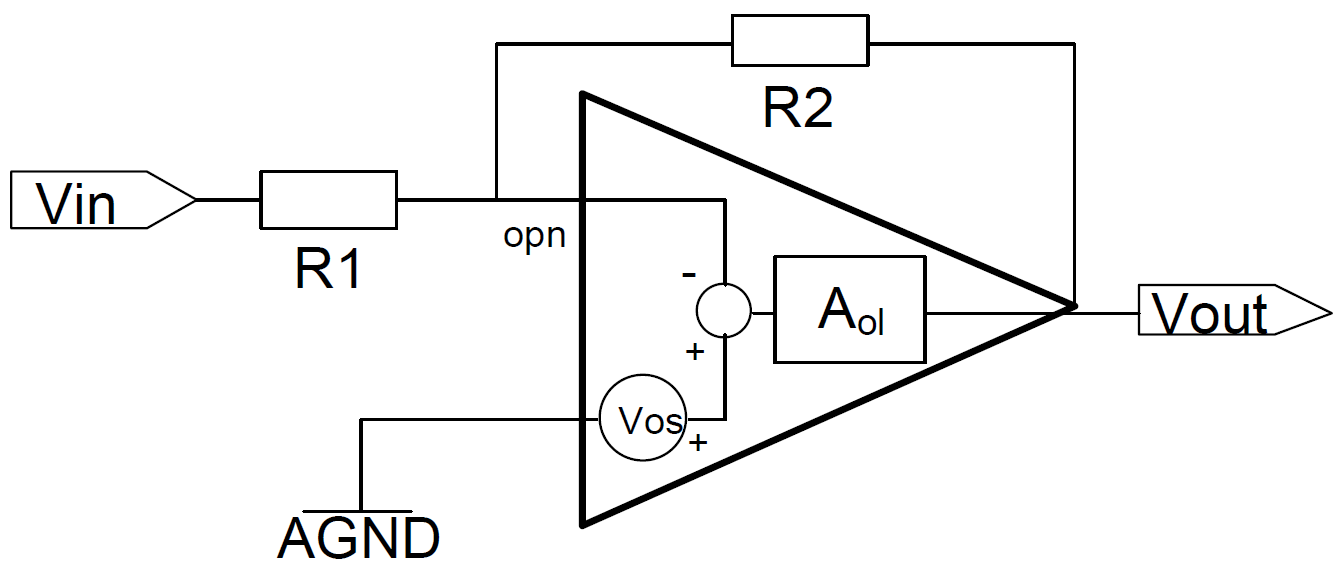
\includegraphics[width=\linewidth,align=c]{images/invertierender_verstaerker_offset.png} &
	\textbf{Invertierend} \quad $Z_{\rm in}=R_1$, \; $G_N = 1+\frac{R_2}{R_1} \neq |A|$ \newline
	$V_{\rm out} = \Big(1+\dfrac{R_2}{R_1}\Big)(V_{\rm AGND}+V_{\rm os}) - \dfrac{R_2}{R_1}V_{\rm in}$ \\
	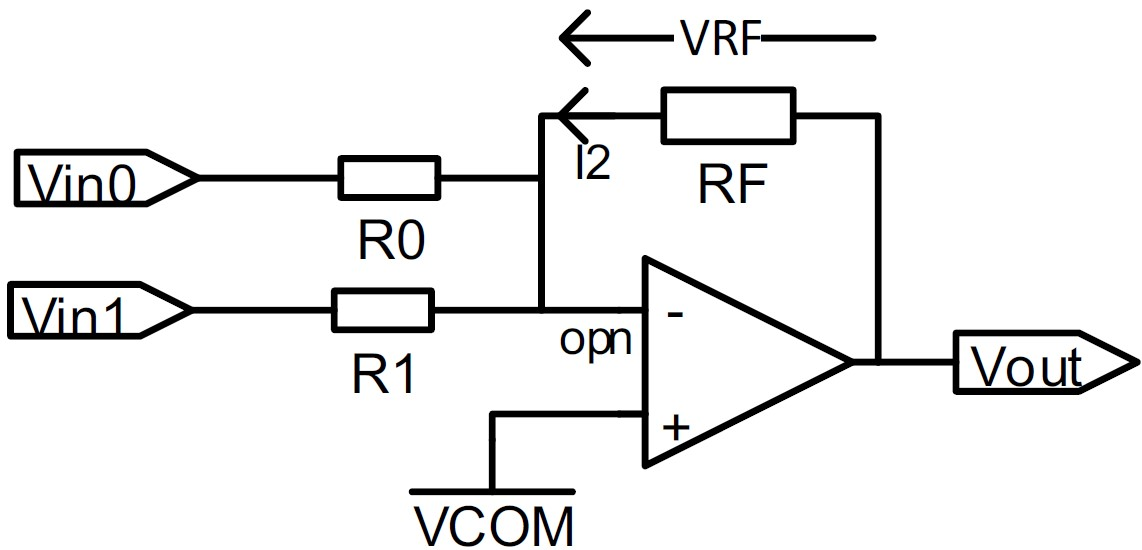
\includegraphics[width=\linewidth,align=c]{images/invertierender_summierender_verstaerker.jpg} &
	\textbf{Addierer} \quad opn = virtuelle Masse \textrightarrow\ Eingänge unabhängig, \; $Z_{\rm in,i}=R_i$ \newline
	$V_{\rm out} = \Big(1+\dfrac{R_F}{R_0\parallel R_1}\Big)(V_{\rm COM}+V_{\rm os}) - R_F\Big(\dfrac{V_{\rm in0}}{R_0}+\dfrac{V_{\rm in1}}{R_1}\Big)$ \\
	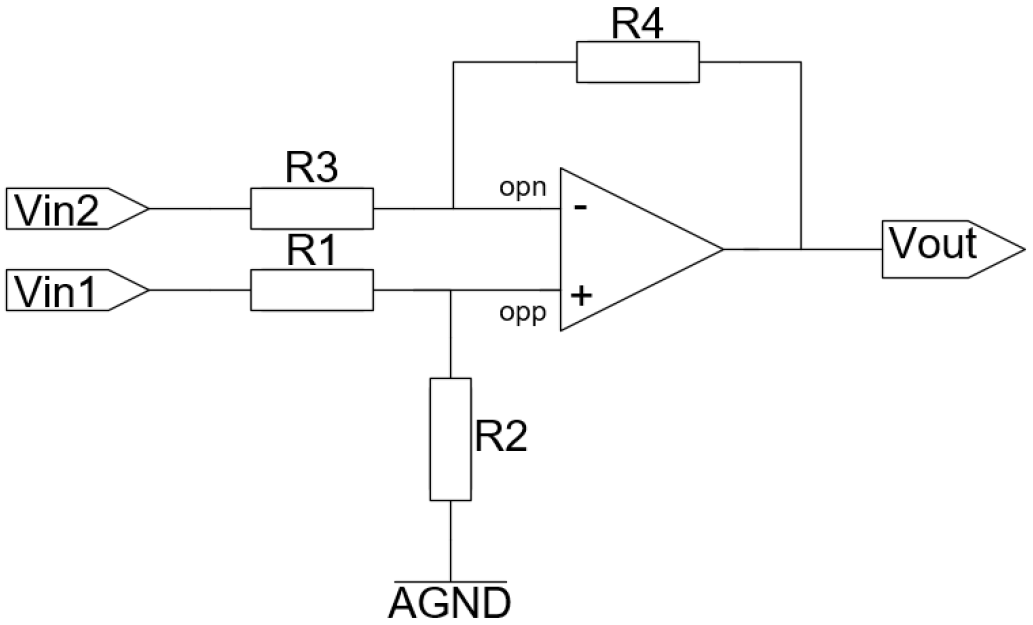
\includegraphics[width=\linewidth,align=c]{images/differenzverstärker.png} &
	\textbf{Subtrahierer} \quad $Z_{\rm in}$ endlich \newline
	$V_{\rm out} = \Big(1+\dfrac{R_4}{R_3}\Big)(V_{\rm opp}+V_{\rm os}) - \dfrac{R_4}{R_3}V_{\rm in2}$, \quad
	$V_{\rm opp} = \dfrac{R_2 V_{\rm in1} + R_1 V_{\rm AGND}}{R_1+R_2}$ \newline
	$R_1{=}R_3,\ R_2{=}R_4$: \; $\boxed{V_{\rm out} = V_{\rm AGND} + \dfrac{R_4}{R_3}(V_{\rm in1}-V_{\rm in2})}$ \; ($A_{\rm CM}=0$) \\
	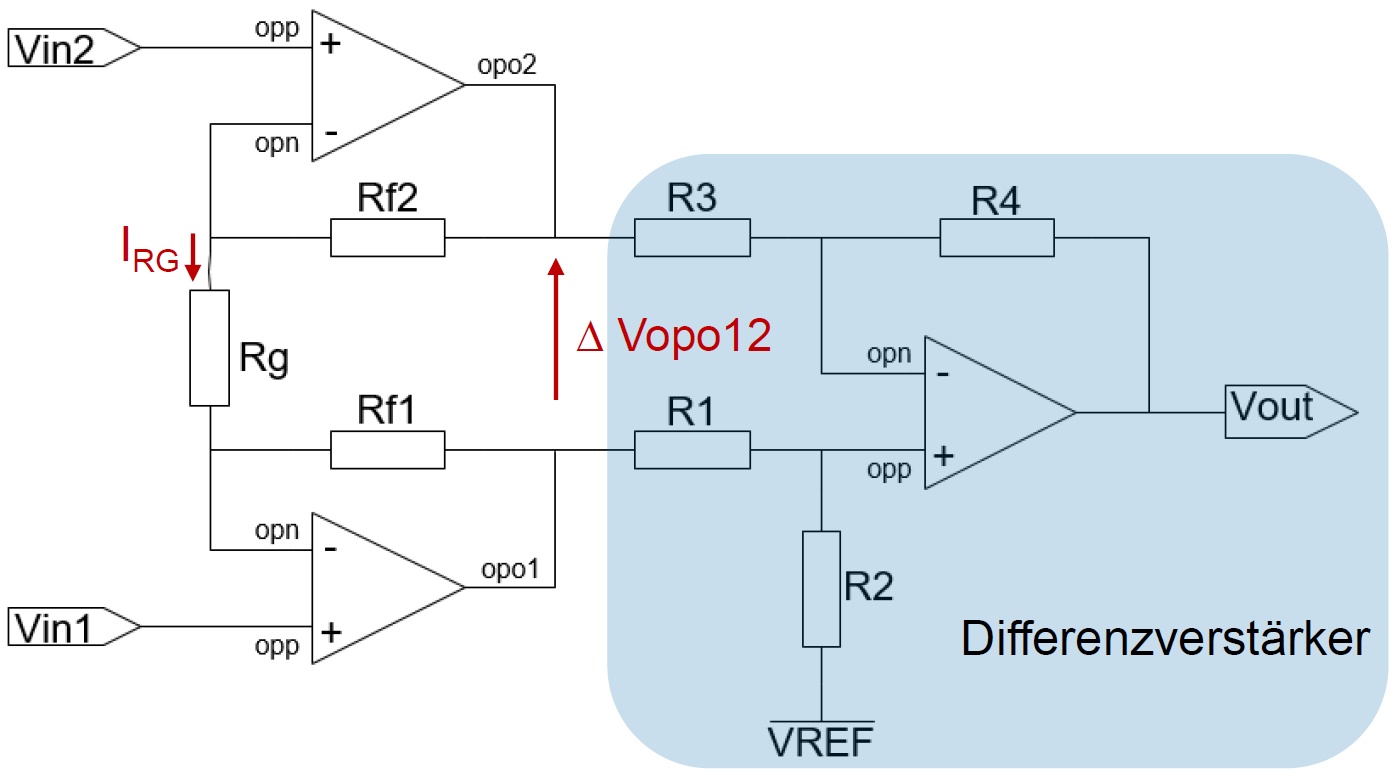
\includegraphics[width=\linewidth,align=c]{images/instrumentenverstaerker.png} &
	\textbf{Instrumentenverstärker} \quad $Z_{\rm in}=\infty$ an beiden Eingängen \newline
	$I_{Rg} = \dfrac{V_{\rm in2}-V_{\rm in1}}{R_g}$ \newline
	$\boxed{V_{\rm out} = V_{\rm REF} + \dfrac{R_4}{R_3}\Big(1+\dfrac{R_{f1}+R_{f2}}{R_g}\Big)(V_{\rm in1}-V_{\rm in2})}$
\end{tabularx}}

\subsubsection*{Weitere Schaltungen}
\vspace{2pt}
{\renewcommand{\arraystretch}{1.6}
\begin{tabularx}{\columnwidth}{@{}l l X@{}}
	\toprule
	\textbf{Schaltung} & \textbf{Formel} & \textbf{Wozu} \\ \midrule
	Geschaltete $R$ & $A_{\rm inv} = -\dfrac{R_f}{R_{\rm var}}$, \; $A_{\rm n.inv} = 1+\dfrac{R_f}{R_{\rm var}}$
	                & $R_{\rm var}$ = Parallelschaltung der \emph{geschlossenen} Zweige \\
	T-Glied         & $A = -\dfrac{R_2R_3+R_2R_4+R_3R_4}{R_1R_4}$
	                & grosse Verstärkung mit kleinen $R$ ($R_2$--$R_3$ zum Ausgang, $R_4$ nach GND) \\
	NIC             & $R_{\rm EQ} = -R\,\dfrac{R_1}{R_2}$
	                & kompensiert die Belastung durch $R_L$ \\ \bottomrule
\end{tabularx}}

\subsection{Nichtidealitäten}\label{sec:opamp-nonideal}

\subsubsection*{Offset-Spannung $V_{\rm os}$}
DC-Quelle in Serie am opp (bis $\pm5\,$mV, jedes IC anders): wird verstärkt wie ein Signal an opp.
$$ \boxed{ \Delta V_{\rm out} = G_N \cdot V_{\rm os} = \Big(1+\frac{R_f}{R_\parallel}\Big) V_{\rm os} } $$
\begin{warnbox}
	\small
	\warn{\textit{Invertente: il segnale ha $-\frac{R_2}{R_1}$, ma $V_{\rm os}$ va $\times\,(1+\frac{R_2}{R_1})$.}}
	\warn{\textit{$R_\parallel$ comprende \textbf{tutte} le R su opn, anche un Poti verso la Speisung.}}
	\warn{\textit{In cascata: $V_{\rm os}$ dello stadio $k$ $\times\, G_N$ dello stadio $k$ $\times$ gain degli stadi dopo.}}
	\warn{\textit{C in serie su opn: in DC è aperto, quindi $G_N=1$ per $V_{\rm os}$.}}
	\warn{\textit{Integratore (C in retroazione): DC-Gain $\infty$, $V_{\rm os}$ viene integrata fino al rail.}}
\end{warnbox}
Kompensation mit Poti an opn ändert auch die Verstärkung \textrightarrow\ besser kalibrieren.

\subsubsection*{Endliche Verstärkung $A_{\rm ol}$}
Schleifenverstärkung $\beta A_{\rm ol}$ mit $\beta = 1/G_N$:
$$ \boxed{ A_{\rm cl} = A_{\rm ideal}\,\frac{\beta A_{\rm ol}}{1+\beta A_{\rm ol}} \approx A_{\rm ideal}\Big(1-\frac{G_N}{A_{\rm ol}}\Big) } $$
$$ \text{nicht-inv.:} \quad V_{\rm out} = \frac{A_{\rm ol}}{1+\beta A_{\rm ol}}\,(V_{\rm in}+V_{\rm os}) $$
\textbf{Exakt}: $V_{\rm opn}$ per Teiler aus $V_{\rm in}$ und $V_{\rm out}$, in die Grundgleichung einsetzen, nach $V_{\rm out}$ auflösen.

\subsubsection*{Eingangsströme $I_B$, $I_{\rm OS}$}
\begin{minipage}[c]{0.36\columnwidth}
	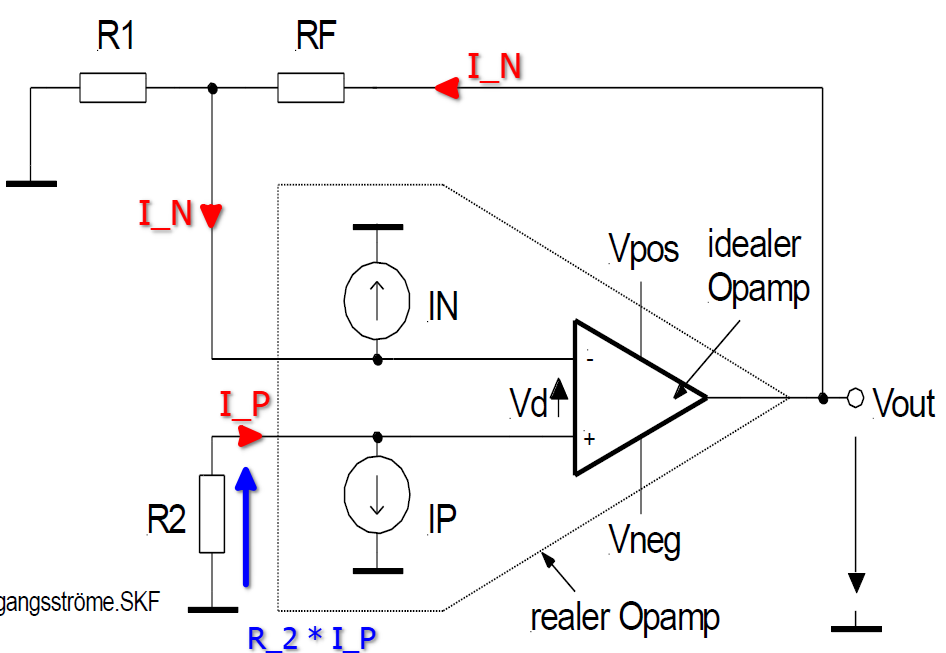
\includegraphics[width=\columnwidth]{images/bias-strom_grafik.png}
\end{minipage}
\hfill
\begin{minipage}[c]{0.62\columnwidth}
	$$ I_B = \frac{I_P+I_N}{2} \qquad I_{\rm OS} = I_P - I_N $$
	$$ V_{\rm outE} = I_N R_F - I_P R_2 \Big(1+\frac{R_F}{R_1}\Big) $$
	Kompensation: \; $\boxed{R_2 = R_F \parallel R_1}$ \; (Buffer: $R_2 = R_F$) \\[3pt]
	Rest: \; $\boxed{V_{\rm outE} = R_F\, I_{\rm OS}}$ \; \textrightarrow\ kleines $R_F$ wählen
\end{minipage}

\subsubsection*{Dynamik: GBW, Slew-Rate, PSRR, CMRR}
\begin{minipage}[c]{0.36\columnwidth}
	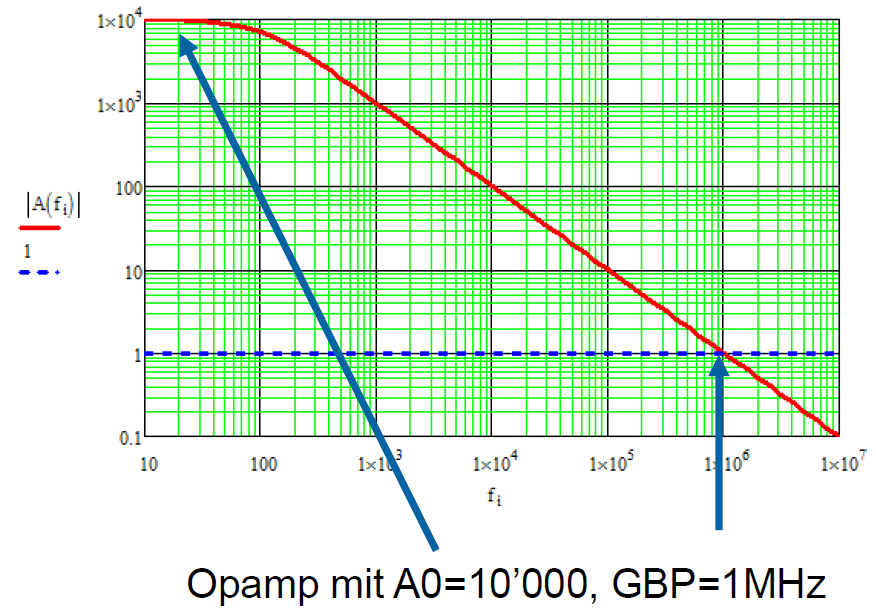
\includegraphics[width=\columnwidth]{images/verstaerkungs-bandbreite-produkt.png}
\end{minipage}
\hfill
\begin{minipage}[c]{0.62\columnwidth}
	$$ A_{\rm ol}(f) = \frac{A_0}{1 + j f A_0/{\rm GBW}} $$
	$$ \boxed{ f_{\rm 3dB} = \beta\cdot{\rm GBW} = \frac{\rm GBW}{G_N} } $$
	\warn{\textit{Conta il Noise Gain: invertente con $A=-10$ ha $G_N=11$ \textrightarrow\ $f_{\rm 3dB}={\rm GBW}/11$.}}
\end{minipage}

\vspace{4pt}
{\renewcommand{\arraystretch}{1.7}
\begin{tabularx}{\columnwidth}{@{}l l X@{}}
	\toprule
	\textbf{Grösse} & \textbf{Definition} & \textbf{Bedeutung} \\ \midrule
	Slew-Rate & ${\rm SR} = \left|\dfrac{\diff V_{\rm out}}{\diff t}\right|_{\max}$
	          & Sinus unverzerrt nur bis $f_{\max} = \dfrac{\rm SR}{2\pi \hat V}$, darüber Dreieck \\
	PSRR      & $\dfrac{\diff V_{\rm supply}}{\diff V_{\rm os}}$
	          & Rippel auf der Speisung wirkt wie ein Offset \\
	CMRR      & $\dfrac{\diff V_{\rm CM}}{\diff V_{\rm os}}$, \; $V_{\rm CM} = \dfrac{V_{\rm opp}+V_{\rm opn}}{2}$
	          & beim invertierenden Verstärker irrelevant \\ \bottomrule
\end{tabularx}}
$$ \boxed{ V_{\rm outE} = G_N\Big(V_{\rm os} + \frac{\Delta V_{\rm CM}}{\rm CMRR} + \frac{\Delta V_{\rm supply}}{\rm PSRR}\Big) + I_{\rm OS} R_F } $$

\subsection{Schaltungen mit Kondensatoren}\label{sec:opamp-C}

\begin{rezept}{Rezept: OpAmp mit $C$ -- DC und AC getrennt}
	\begin{steps}
		\item \textbf{DC}: $C$ offen \textrightarrow\ $V_{\rm out,DC}$ (mit $V_{\rm os}$ und dem $G_N$ \emph{ohne} $C$-Zweige)
		\item \textbf{AC}: $C$ Kurzschluss (prüfen: $f \gg f_g = \frac{1}{2\pi RC}$), DC-Quellen $=0$ \textrightarrow\ $A_{\rm AC}$
		\item Zusammensetzen, dann prüfen: bleiben die Spitzen innerhalb der Rails?
	\end{steps}
	$$ v_{\rm out}(t) = V_{\rm out,DC} + A_{\rm AC}\,\hat v \sin(2\pi f t) $$
\end{rezept}
\textbf{Rippel auf der Speisung} über einen Teiler an opp: wirkt wie ein Eingang
$$ v_{\rm out} = v_{\rm pos}\,\frac{R_3}{R_3+R_4}\,G_{N,\rm AC} $$

\vspace{3pt}
\begin{minipage}[t]{0.24\columnwidth}\centering
	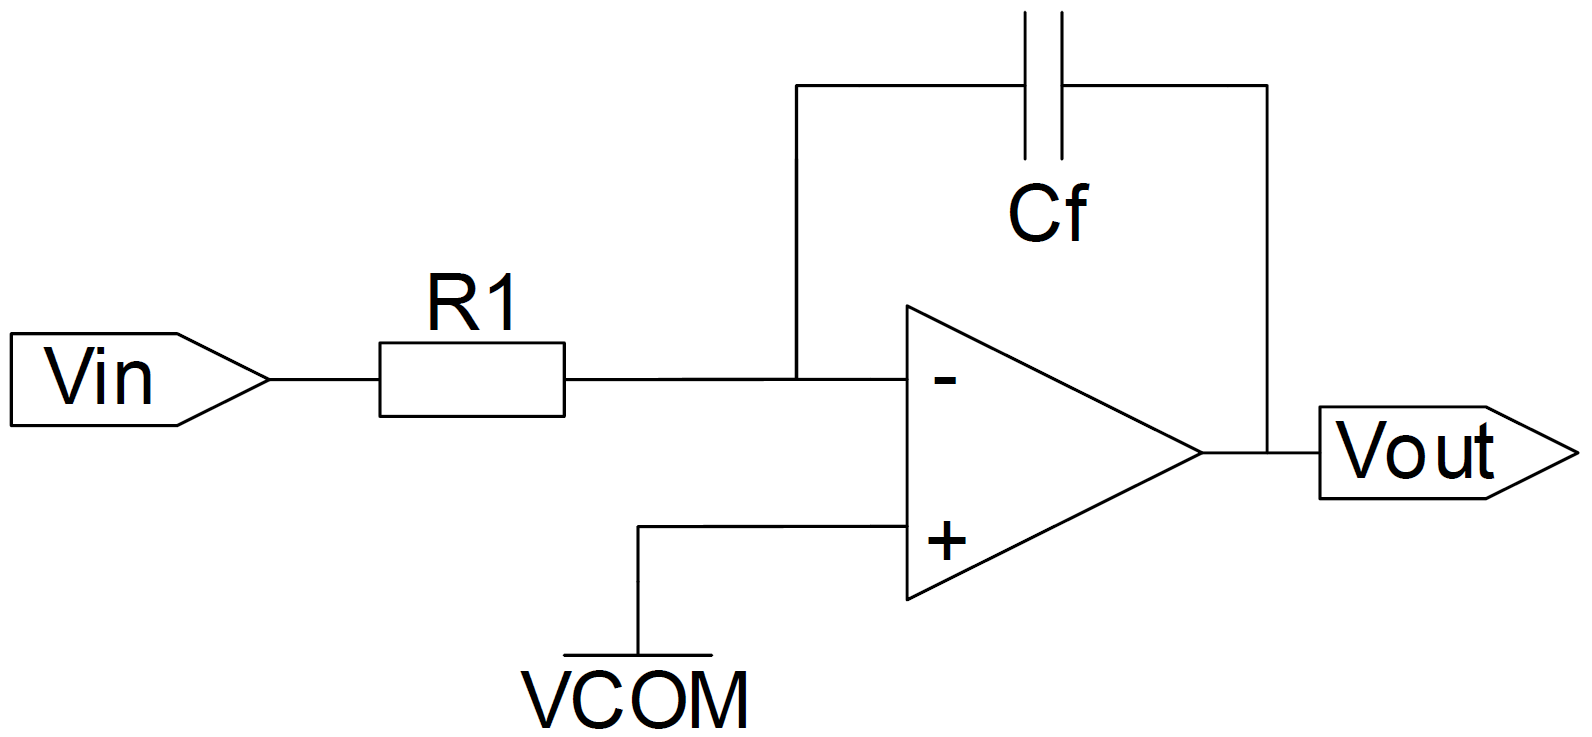
\includegraphics[width=\columnwidth]{images/integrator.png}\\[-1pt]{\scriptsize Integrator}
\end{minipage}\hfill
\begin{minipage}[t]{0.24\columnwidth}\centering
	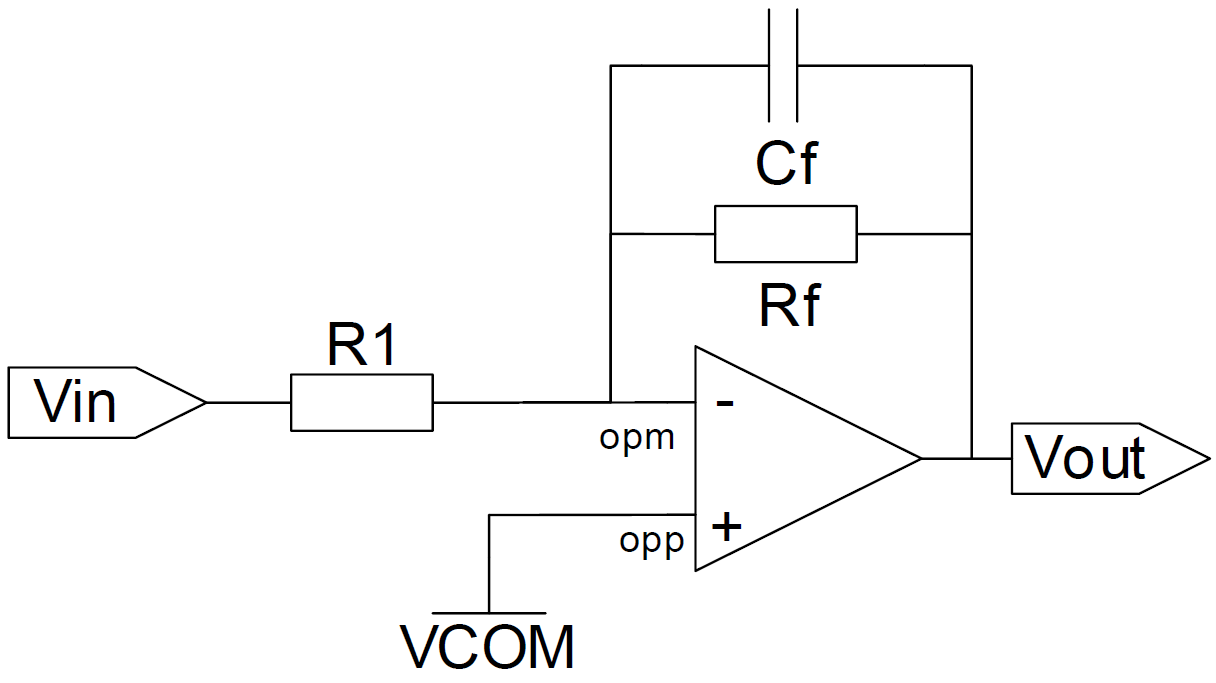
\includegraphics[width=\columnwidth]{images/tiefpass.png}\\[-1pt]{\scriptsize Tiefpass}
\end{minipage}\hfill
\begin{minipage}[t]{0.24\columnwidth}\centering
	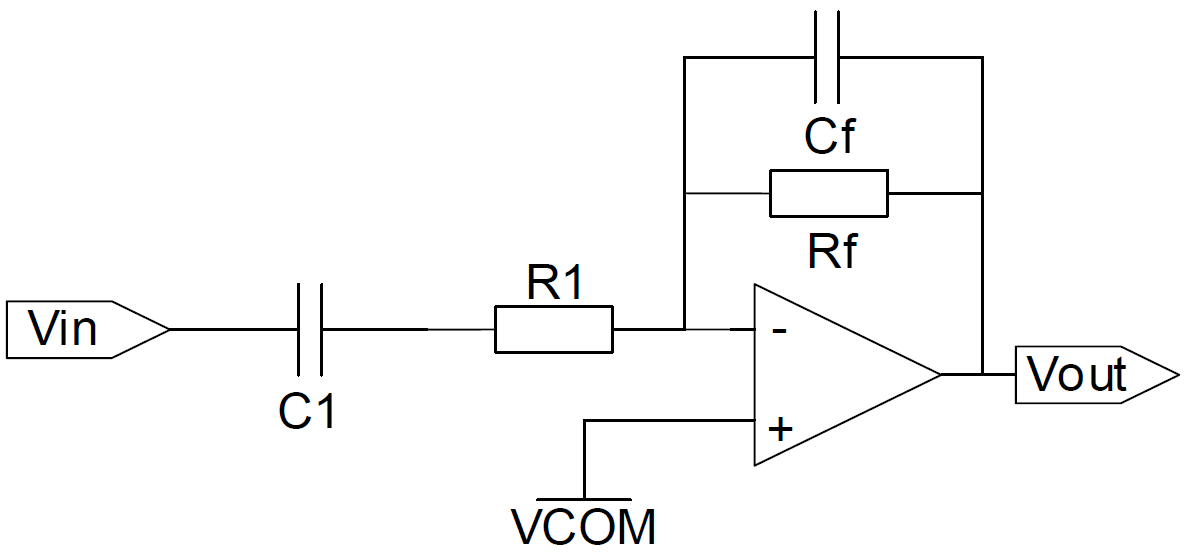
\includegraphics[width=\columnwidth]{images/bandpass.png}\\[-1pt]{\scriptsize Bandpass}
\end{minipage}\hfill
\begin{minipage}[t]{0.24\columnwidth}\centering
	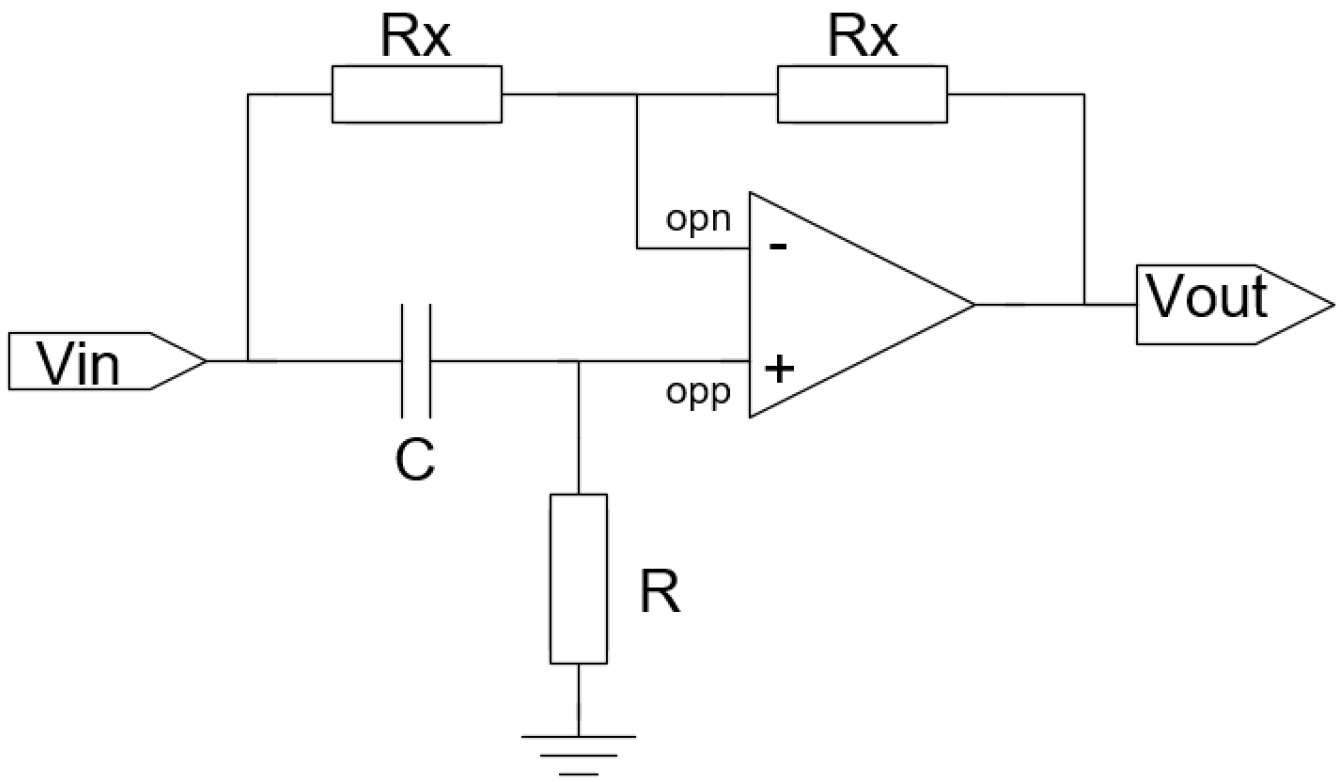
\includegraphics[width=\columnwidth]{images/allpass.png}\\[-1pt]{\scriptsize Allpass}
\end{minipage}

{\small
\renewcommand{\arraystretch}{1.3}
\begin{tabularx}{\columnwidth}{@{}l l >{\raggedright\arraybackslash}X >{\raggedright\arraybackslash}X@{}}
	\toprule
	& $Z_1$ / $Z_f$ & \cbl{tiefe $f$} / \cgn{hohe $f$} & Formel \\ \midrule
	Integrator     & $R_1$ / $C_f$                    & \cbl{Gain $\to\infty$ ($V_{\rm os}$!)} \newline \cgn{$-20\,$dB/Dek}
	               & $V_{\rm out} = V_0 - \frac{1}{R_1C_f}\!\int\!(V_{\rm in}-V_{\rm COM})\,\diff t$ \\
	Differenzierer & $C_1$ / $R_f$                    & \cbl{$0$} \newline \cgn{$+20\,$dB/Dek, Rauschen, schwingt}
	               & $V_{\rm out} = -R_f C_1 \frac{\diff V_{\rm in}}{\diff t}$ \\
	Tiefpass       & $R_1$ / $R_f\parallel C_f$       & \cbl{$-\frac{R_f}{R_1}$} \newline \cgn{wie Integrator}
	               & $f_g = \frac{1}{2\pi R_f C_f}$ \\
	Bandpass       & $R_1{+}C_1$ / $R_f\parallel C_f$ & \cbl{wie Differenzierer} \newline \cgn{wie Integrator}
	               & $\omega_1 = \frac{1}{R_1C_1}$, $\omega_2 = \frac{1}{R_fC_f}$ \newline Mitte $-\frac{R_f}{R_1}$ \\
	Allpass        & $R_x$ / $R_x$, $RC$ an opp       & \cbl{$-V_{\rm in}$} \newline \cgn{$+V_{\rm in}$}
	               & $|H|=1$ \newline $\varphi = 180\degree - 2\arctan(\omega RC)$ \\ \bottomrule
\end{tabularx}
\renewcommand{\arraystretch}{1}
}

\vspace{4pt}
\textbf{Integrator mit konstantem $V_{\rm in}$}: lineare Rampe (\textrightarrow\ Oszillator Kap.~3, Dual-Slope Kap.~5)
$$ \boxed{ V_{\rm out}(t) = V_{\rm out}(0) - \frac{V_{\rm in}-V_{\rm COM}}{R_1 C_f}\; t } \qquad I_C = \frac{V_{\rm in}-V_{\rm COM}}{R_1} $$

\subsection{Mehrstufige Verstärker}\label{sec:opamp-kaskade}

\begin{center}
	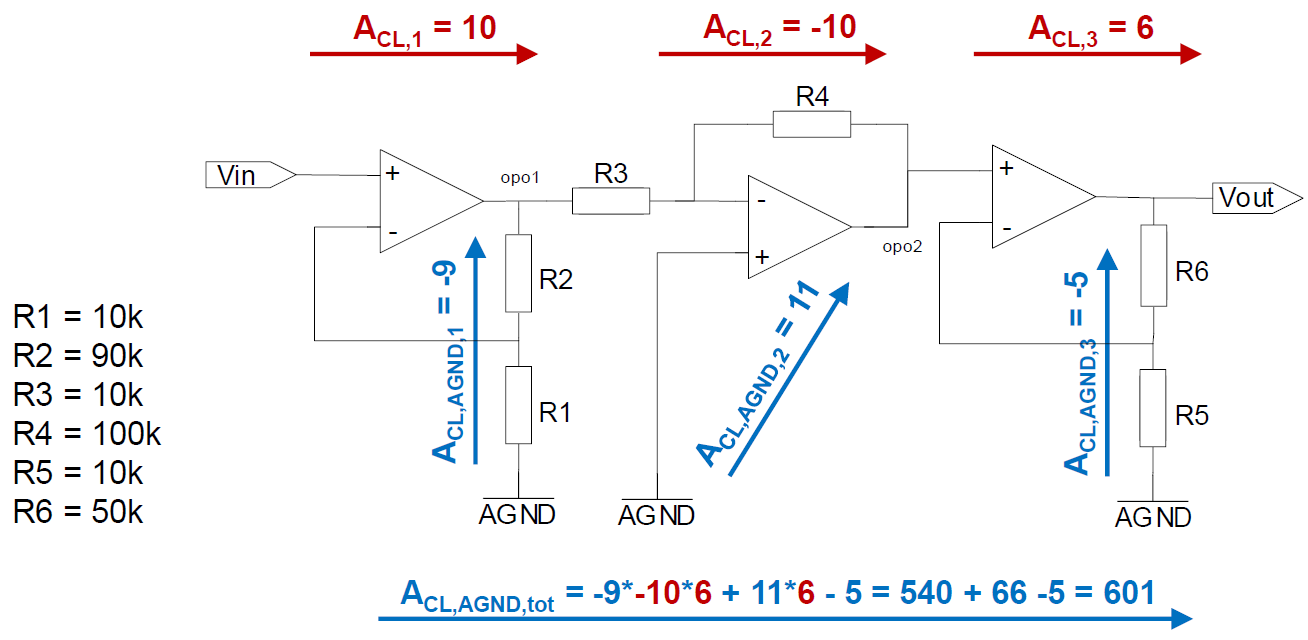
\includegraphics[width=0.8\columnwidth]{images/mehrstufige_verstaerker.png}
\end{center}

\begin{rezept}{Rezept: Kaskade mit Referenzen ($V_{\rm ref}$, AGND $\neq 0$)}
	\begin{steps}
		\item Jede Stufe als $V_{{\rm out},k} = a_k V_{{\rm in},k} + b_k$ schreiben (Rezept \ref{sec:opamp-rezept})
		\item Von hinten einsetzen: die Gains multiplizieren sich, jede Referenz läuft durch alle \emph{folgenden} Stufen
	\end{steps}
	$$ V_{\rm out} = a_2(a_1 V_{\rm in} + b_1) + b_2 = a_1 a_2\, V_{\rm in} + a_2 b_1 + b_2 $$
\end{rezept}

\subsection{Gesteuerte Quellen}

\begin{minipage}[t]{0.3\columnwidth}\centering
	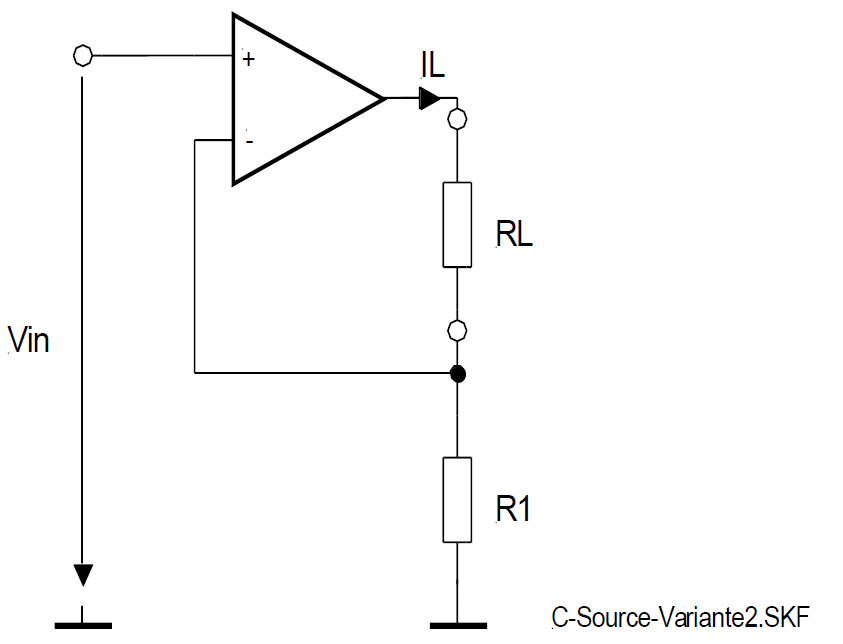
\includegraphics[width=0.75\columnwidth]{images/spannungsgesteuerte_stromquelle_V1.png}
	$I_L = \dfrac{V_{\rm in}}{R_1}$ \\ {\scriptsize Last «floating»}
\end{minipage}\hfill
\begin{minipage}[t]{0.3\columnwidth}\centering
	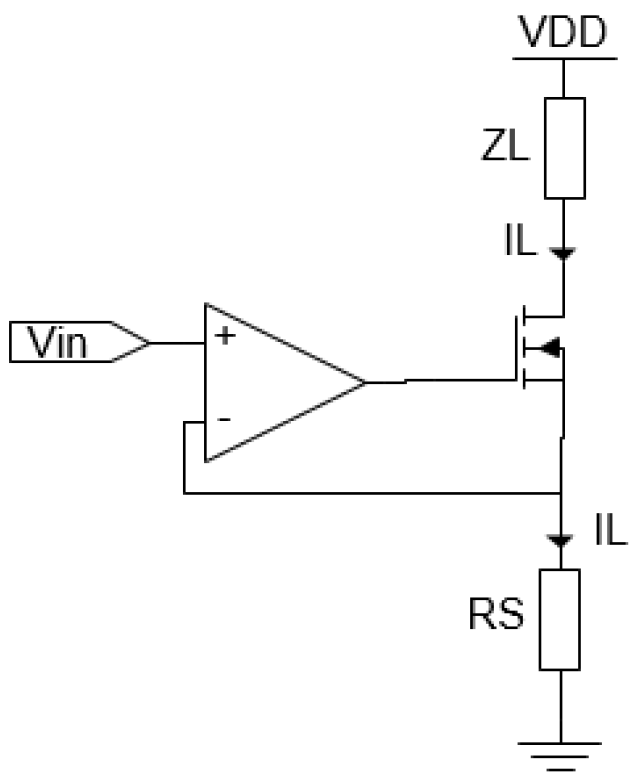
\includegraphics[width=0.6\columnwidth]{images/spannungsgesteuerte_stromquelle_V2.png}
	$I_L = \dfrac{V_{\rm in}}{R_S}$ \\ {\scriptsize Last an $V_{\rm DD}$}
\end{minipage}\hfill
\begin{minipage}[t]{0.36\columnwidth}\centering
	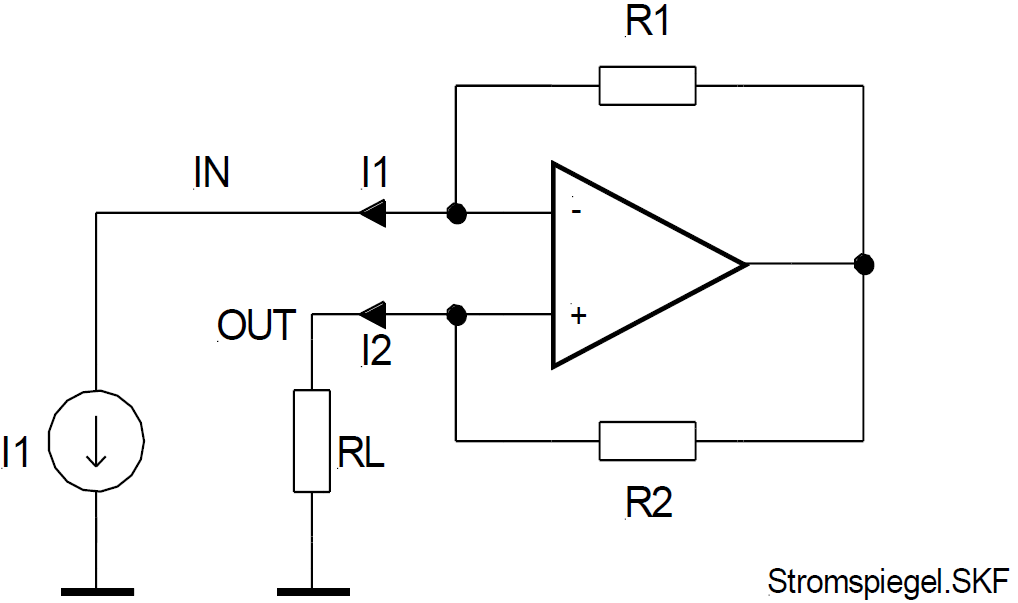
\includegraphics[width=0.85\columnwidth]{images/stromspiegel_OPV.png}
	$A_i = \dfrac{I_2}{I_1} = \dfrac{R_1}{R_2}$ \\ {\scriptsize stromgesteuert}
\end{minipage}

\vspace{4pt}
\textbf{Stromquelle mit BJT} ($V_{\rm ref}$ an opp, Emitter an opn über $R_E$):
$$ I = \frac{V_{\rm ref}}{R_E} \qquad V_{\rm opo} = V_{\rm ref} + V_{\rm BE} \qquad V_{\rm out} = V_0 - I Z_L $$
